% !TeX root = ../libro.tex
% !TeX encoding = utf8

\setchapterpreamble[c][0.75\linewidth]{%
	\sffamily
  Definiremos los modelos utilizados en el trabajo. 
	\par\bigskip
}
\chapter{Aprendizaje automático}\label{ch:machine-learning}
El aprendizaje automático es una aplicación de la inteligencia artificial hace uso de los algoritmos de aprendizaje que estiman una dependencia desconocida entre los datos de entrada y de salida de un sistema desde unas muestras conocidas. Una vez esta dependencia ha sido estimada, se puede usar para predecir las futuras salidas del sistema a partir de los valores de entrada conocidos.\\
Hay tres tipos de aprendizajes:
\begin{itemize}
  \item Aprendizaje \textbf{supervisado}: Es el tipo de aprendizaje más utilizado. Se aplica a datos \textbf{etiquetados}. Tiene como objetivo aprender la función desconocida que asigna los datos con las etiquetas minimizando una función de error. lo usaremos para nuestro conjunto de datos, pues es etiquetado.
  \item Aprendizaje \textbf{no supervisado}: Se usa para los datos no etiquetados y se pretende buscar patrones o relaciones entre los datos. Un ejemplo típico de este tipo de aprendizaje es el de \textbf{agrupamiento} o \textit{clustering} que busca agrupar los datos según algún patrón o relación.
  \item Aprendizaje \textbf{por refuerzo}: En vez de ser etiquetado, da solo una indicación de si la predicción es correcta o no mediante alguna recompensa o penalización en función de las acciones que haga.
\end{itemize}
\cite{jordan2015machine}\\
\section{Esquema básico de aprendizaje}
Un primer ejemplo y esquema de aprendizaje automático sería el siguiente, supongamos que hay un banco que recive miles de solicitudes para una tarjeta de crédito y quiere automatizar el proceso. No se conoce ninguna fórmula para aceptar o denegar una tarjeta pero se dispone de gran cantidad de datos de los aplicantes: información personal, sueldo, prestamos pendientes y más información relacionada al crédito, así que se usan estos datos para encontrar una fórmula adecuada.\\
Así, se tiene la entrada \textbf{x} (información del cliente), la función desconocida ideal para llevar a cabo la decisión $f:X \rightarrow Y$, donde $X$ es el espacio de la entrada (conjunto de las posibles entradas de \textbf{x}), e $Y$ es el espacio de la salida (conjunto de todas las posibles salidas, en este caso una decisión de sí o no). Se denotará al set de datos por $D$, con ejemplos de entrada-salida $(x_{1},y_{1}),...,(x_{N},y_{N})$ donde $y_{n}=f(x_{n})$ para $n=1,...,N$. Los ejemplos se suelen llamar muestras. Por último, hay un algoritmo de aprendizaje que aproxima $h:X \rightarrow Y$ a $f$.  El algoritmo elige $h$ de entre un conjunto de funciones candidatas o hipótesis, $H$, como por ejemplo el conjunto de todas las funciones lineales.\\
El banco usará la función $h$ para hacer la decisión puesto que la $f$ ideal no la tiene así que el algoritmo elige la $h$ que mejor aproxima $f$ en un conjunto de \textit{entrenamiento} o \textit{training} de anteriores clientes. \cite{abu2012learning}\\
La siguiente figura ilusta esquemáticamente el problema de aprendizaje:
\begin{figure}[H]
  \centering
  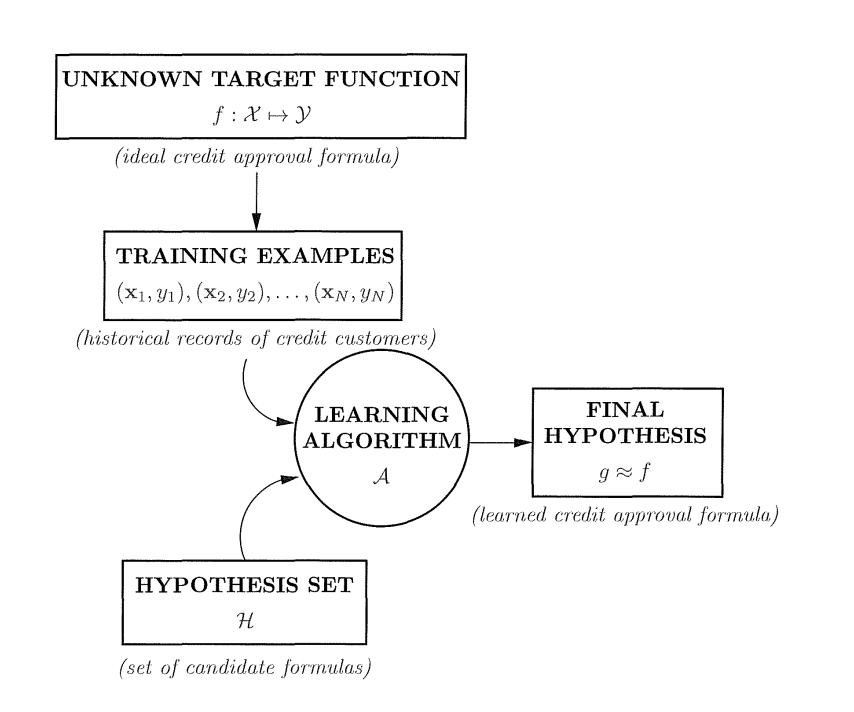
\includegraphics[width=0.65\textwidth]{Problema_aprendizaje_basico}
  \caption{Esquema básico de aprendizaje. \cite{abu2012learning}}
  \label{fig:k-nn-example}
\end{figure}

Para este trabajo, $X=\mathbb{R}^{d}$, siendo $\mathbb{R}^{d}$ un espacio euclídeo d-dimensional, con las coordenadas descritas en el \autoref{ch:base-datos} siendo cada columna una coordenada, $Y=\lbrace 0,2 \rbrace$ una decisión binaria de si el individuo es sano o afectado (o padre de afectado para el estudio con controles).\\
\section{Errores}
También hay que tener en cuenta dos conceptos importantes: los errores o funciones de pérdida. Hay de dos tipos, el primero es el error dentro de la muestra definido como la fracción de $D$ donde $f$ y $h$ no concuerdan:
\[E_{in}(h) = \frac{1}{N}\sum_{n=1}^{N}[[h(x_{n}) \neq f(x_{n})]]\]
donde el operador [[$\cdot$]]=1 si lo de dentro se cumple y 0 en caso contrario. Análogamente también está el error fuera de la muestra:
\[ E_{out}(h)=\mathbb{P}[h(x) \neq f(x)] \]
la probabilidad está basada en la distribución de $X$ que se usa para muestrear.\\
Para cuantificar la relación que existe entre estos dos errores se usa la \textit{desigualdad de Hoeffding}, que provee de una cota superior de la probabilidad de que la suma de variables aleatorias independientes y acotadas se desvíe de su valor esperado más de una cierta cantidad. Esta desigualdad indica que para cualquier tamaño de muestra N,
\[ \mathbb{P}[\vert E_{in}(h)-E_{out}(h) \vert > \epsilon] \leq  2e^{-2\epsilon^{2}N} \quad \forall \epsilon > 0 \]
El error dentro de la muestra $E_{in}$ es una variable aleatoria que depende de la muestra y el error fuera de la muestra $E_{out}$ es desconocido pero no aleatorio. Ahora bien, esto ocurre bajo el supuesto de que $h$ está fija y es una en particular antes de generar el conjunto de datos. \cite{abu2012learning}
\subsection{Generalización de errores I}
Para solucionar que $h$ tenga que estar \textbf{fija}, consideramos un conjunto de hipótesis $H$ y asumimos primero que tien un número finito de hipótesis $H=\lbrace h_{1},...,h_{M}$. El objetivo es poder poner el límite a una hipótesis $g$ de $H$ que no esté fija antes de generar los datos, porque la hipótesis seleccionada $g$ depende de los datos. Así que vamos a intentar limitar $\mathbb{P}[\vert E_{in}(g)-E_{out}(g) \vert > \epsilon]$ de forma que no dependa de la $g$ que el algoritmo de aprendizaje elija. Como $g$ es una de las hipótesis independientemente del algoritmo y de la muestra, siempre es verdad que:
"$\vert E_{in}(g)-E_{out}(g) \vert > \epsilon$" $\Longrightarrow$ "$\vert E_{in}(h_{1})-E_{out}(h_{1}) \vert > \epsilon$ \textbf{or} $\vert E_{in}(h_{2})-E_{out}(h_{2}) \vert > \epsilon$ \textbf{or} ... \textbf{or} $\vert E_{in}(h_{M})-E_{out}(h_{M}) \vert > \epsilon$".\\
Llamemos $\mathcal{B}_{1}$ a la parte izquierda de la implicación anterior y $\mathcal{B}_{2}$ a la parte derecha.$\mathcal{B}_{2}$ tiene la propiedad deseada: las hipótesis $h_{m}$ están fijas, y aplicamos dos reglas básicas de probabilidad:
\[ \textnormal{si } \mathcal{B}_{1} \Longrightarrow \mathcal{B}_{2} \textnormal{ entonces } \mathbb{P}[\mathcal{B}_{1}] \leq \mathbb{P}[\mathcal{B}_{2}]\]
y que si $\mathcal{B}_{1},\mathcal{B}_{2},...,\mathcal{B}_{M}$ son cualesquiera eventos, entonces:
\[ \mathbb{P}[\mathcal{B}_{1} \textnormal{ or } ... \textnormal{ or } \mathcal{B}_{M}] \leq \mathbb{P}[\mathcal{B}_{1}]+...+\mathbb{P}[\mathcal{B}_{M}] \]
Tenemos con estas dos propiedades que:
\[ \mathbb{P}[\vert E_{in}(g)-E_{out}(g) \vert > \epsilon] \leq \mathbb{P}[\vert E_{in}(h_{1})-E_{out}(h_{1}) \vert > \epsilon \textnormal{\textbf{ or }} \vert E_{in}(h_{2})-E_{out}(h_{2}) \vert > \epsilon \textnormal{\textbf{ or }} ...\]
\[\textnormal{\textbf{ or }} \vert E_{in}(h_{M})-E_{out}(h_{M}) \vert > \epsilon] \leq \sum_{m=1}^{M}\mathbb{P}[\vert E_{in}(h_{m})-E_{out}(h_{m}) \vert > \epsilon] \]
Aplicando la desigualdad de Hoeffding a los M términos de la sumatoria obtenemos el resultado deseado:
\[ \mathbb{P}[\vert E_{in}(g)-E_{out}(g) \vert > \epsilon] \leq 2Me^{-2\epsilon^{2}N} \]
Como se puede ver, esto funciona cuando M es finita. \cite{abu2012learning}
\subsection{Generalización de errores II}
Para terminar esta sección se va a definir la \textit{función de crecimiento} o, más conocida en inglés, \textbf{\textit{growth function}} que formaliza el número efectivo de hipótesis.\\
Antes vamos a convertir la formula $\mathbb{P}[\vert E_{in}(g)-E_{out}(g) \vert > \epsilon] \leq 2Me^{-2\epsilon^{2}N}$ en algo más conveniente. Tomamos un \textit{nivel de tolerancia} $\delta$ y afirmamos con una probabilidad de al menos $1 - \delta$ que:
\[ E_{out} \leq E_{in}(g) + \sqrt{\frac{1}{2N} ln \frac{2M}{\delta}} \] 
A esta cota se la llama \textit{cota de generalización} pues acota $E_{out}$ en términos de $E_{in}$. Se ha conseguido la expresión de la siguiente forma: con al menos una probabilidad de $1 - 2Me^{-2N \epsilon^{2}}$, $\vert E_{out} - E_{in} \vert \leq \epsilon $ lo que implica que $E_{out} \leq E_{in} + \epsilon$. Escribimos $\delta = 2Me^{-2N\epsilon^{2}}$, de donde $\epsilon=\sqrt{\frac{1}{2N}ln\frac{2M}{\delta}}$ y se deduce la cota de generalización.
\begin{definicion}
Sean $x_{1},...,x_{N} \in X$. La dicotomía generada por H en estos puntos está definida por  \[ H(x_{1},...,x_{N})= \lbrace (h(x_{1}),...,h(x_{n})) \vert h \in H \rbrace \]
\end{definicion}
Es una dicotomía pues separa $x_{1},...,x_{n}$ en dos grupos: los que su $h$ vale 1 y los que vale -1, así, cuanto mayor es la dicotomía, más 'diversa' es $H$.
\begin{definicion}
La \textbf{función de crecimiento} está definida por un conjunto de hipótesis $H$ por \[ m_{H}(N)=\max_{x_{1},...,x_{N} \in X} \vert H(x_{1},...,x_{N}) \vert \]
donde $\vert \cdot \vert$ indica la cardinalidad del conjunto.
\end{definicion}
En otras palabras, $m_{H}(N)$ es el máximo número de dicotomías que pueden ser generadas por $H$ en cualquiera $N$ puntos.\\
Para cualquier $H$, como $H(x_{1},...,x_{N}) \subseteq \lbrace -1,+1 \rbrace$, el valor de $m_{H}(N)$ es como mucho $\vert \lbrace -1,+1 \rbrace \vert$, así que $m_{H}(N) \leq 2^{N}$. Por intuición se puede afirmar que $m_{H}(N)$ crece más rápido cuanto más compleja se vuelve $H$, que es lo que se espera ya que es lo que va a reemplazar a M en la cota de generalización. Si $H$ es capaz de generar todas las posibles dicotomías en la muestra, se dice que \textit{separa}, o en inglés \textbf{\textit{shatter}}, $x_{1},...,x_{N}$\\
Sin embargo, no es práctico computar $m_{H}$ para cada conjunto de hipótesis que se use, pero esto no es necesario pues basta con usar una cota superior y la cota de generalización aún se sostendrá y así se hará más facil computar $m_{H}$.
\begin{definicion}
Si el conjunto nungún conjunto de datos de tamaño k puede ser \textit{separado} por $H$, entonces k se dice que es un \textbf{punto de ruptura} para $H$.
\end{definicion}
\cite{abu2012learning}\\
Así, $m_{H} < 2^{k}$ y en general es más fácil de encontrar este punto que de computar la función de crecimiento completa para esa $H$. Lo más importante de este concepto es que si $m_{H}(N)=2^{N}$ rompe en cualquier punto, podemos acotar $m_{H}$ por un polinomio de forma que si se sustituye por $M$ en el \textit{error de generalización} $\sqrt{\frac{1}{2N}ln\frac{2M}{\delta}}$ cuando $N \longrightarrow \infty$ irá a cero, cosa que no pasa sin esa cota polinómica.\\
Ahora se va a probar esa cota polinómica. Introducimos antes un concepto. No depende de $H$ así que la cota será aplicada a cluaquier $H$.
\begin{definicion}
Se denota $B(N,k)$ al número máximo de dicotomías en $N$ puntos tales que ningún subconjunto de tamaño $k$ del de $N$ puntos puede ser \textit{separado} por estas dicotomías.
\end{definicion}
Esta definición asume un punto de ruptura $k$ y está definido como un máximo así que sirve como cota superior para cualquier $m_{H}(N)$ que tenga un punto de ruptura $k$:
\[ m_{H}(N) \leq B(N,k) \textnormal{ si } k \textnormal{ es un punto de ruptura para } H\]
\begin{lema}
(Lema de Sauer) \[ B(N,k) \leq \sum_{i=0}^{k-1} \binom{N}{i} \]
\end{lema}
\begin{proof}
Cuando $k=1$, $B(N,1)=1$ para todo $N$ pues ningún subconjunto de tamaño 1 puede ser separado así que sólo admite una dicotomía así que el lema se cumple. Cuando $N=1$, $B(1,k)=2$ para $k>1$ puesto que no existen subconjuntos de tamaño $k$ así que las dos únicas posibilidades son 1 y -1, con lo que el lema se cumple. Ahora se va a realizar la prueba por inducción, asumimos que es cierto para todo $N \leq N_{0}$ y todo $k$. Necesitamos probar que es verdad para $N=N_{0}+1$ y todo $k$. Como la desigualdad ya es cierta cuando $k=1$ solo hace flata preocuparse por $k \geq 2$. Por definición de B, ocurre que
\[ B(N_{0}+1,k) \leq B(N_{0},k)+B(N_{0},k-1) \]
Aplicando la hipótesis de inducción a cada término de la derecha de la desigualdad se tiene que:
\[ B(N_{0}+1,k) \leq \sum_{i=0}^{k-1} \binom{N_{0}}{i} + \sum_{i=0}^{k-2} \binom{N_{0}}{i} =\] \[ = 1 + \sum_{i=0}^{k-1} \binom{N_{0}}{i} + \sum_{i=0}^{k-1} \binom{N_{0}}{i-1} = 1+ \sum_{i=0}^{k-1} \left[ \binom{N_{0}}{i} + \binom{N_{0}}{i-1} \right] = \] \[ = 1 + \sum_{i=0}^{k-1} \binom{N_{0} + 1}{i} = \sum_{i=0}^{k-1} \binom{N_{0}+1}{i}\]
donde se ha usado la identidad de combinatoria $\binom{N_{0}+1}{i} = \binom{N_{0}}{i}+\binom{N_{0}}{i-1}$. Probado esto, la inducción concluye y el lema es cierto para todo $N$ y $k$.
\end{proof}
Como $B(N,k)$ es una cota superior para $M_{H}(N)$, el siguiente teorema está desmotrado:
\begin{teorema}\label{th:th3.1}
Si $m_{H}(k)<2^{k}$ para algún k, entonces
\[ m_{H}(N) \leq \sum_{i=0}^{k-1} \binom{N}{i} \]
para todo $N$.
\end{teorema}
Así, tenemoos una cota polinómica de grado $k-1$ para $m_{H}(N)$.\cite{abu2012learning}\\\\
Ahora presentamos una nueva definición qeu caracterizará a la función de crecimiento.
\begin{definicion}
La \textbf{dimensión Vapnik-Chervonenkis} de un conjunto de hipótesis $H$, denotado por $d_{VC}(H)$ o simplemente $d_{VC}$, es el mayor valor de $N$ para el que $m_{H}(N)=2^{N}$. Si $m_{H}(N)=2^{N}$ para todo $N$, entonces $d_{VC}(H)=\infty$.
\end{definicion}
Si $d_{VC}$ es la dimensión VC de $H$, entonces $k=d_{VC}+1$ es un punto de ruptura para $m_{H}$. Por tanto, podemos escribir el \autoref{th:th3.1} como:
\[  m_{H}(N) \leq \sum_{i=0}^{d_{VC}} \binom{N}{i} \]
Y la dimensión VC es el orden de la cota polinómica.\\
Para terminar la sección, vamos a introducir la cota donde se reemplaza $M$ por $m_{H}(N)$ con ciertos ajustes, el resultado matemático más importante de la teoría de aprendizaje. \cite{abu2012learning}\\
Denotemos $P_{xy}$ a la distribución que sigue cada $(x,y)$ de $D$. Para la demostración se usarán las etiquetas 0 y 1 en vez de -1 y 1.
\begin{teorema}
\textbf{Cota de generalizazión VC}. Para una clasificación binaria tenemos y una función de pérdida (o error):
\[ P \left( \sup_{h \in H} \vert E_{in}(h)-E_{out}(h) \vert > \epsilon \right) \leq 8m_{H}(N)e^{-N \epsilon^{2}/32} \textnormal{ ,} \]
y
\[ E \left[ \sup_{h \in H} \vert E_{in}(h)-E_{out}(h) \vert \right] \leq 2 \sqrt{\frac{log(m_{H}(N))+log2}{N}} \]
\end{teorema}
\begin{proof}
La segunda expresión es consecuencia directa de la primera, así que vamos a demostrar la primera.\\
La prueba consistirá en varios pasos. Se usará para la demostración una \textit{"muestra fantasma"} para ayudar a desarrollarla pero no jugará ningún papel en el resultado final, es decir, no se necesita esa muestra fantasma para aplicar el resultado. La definimos como $D'=\lbrace(x'_{1},y'_{1}),...,(x'_{n},y'_{n})\rbrace$, un conjunto de variables aleatorias independientes de $D_{n}$ tales que $(x'_{i},y'_{i})\sim^{i.i.d.} P_{xy}$. El error bajo esta muestra es:
\[ E'_{in}(h)=\frac{1}{N}\sum_{i=0}^{N}[[h(x'_{i}) \neq y'_{i}]] \] 
Para el resto de la demostración asumiremos que $N\epsilon^{2} \geq 2$ sin pérdida de genereladidad pues de otra forma, la cota sería trivial.\\
\textbf{Paso 1:} Primera simetrización por una muestra fantasma:\\
Mostraremos que 
\[ P \left( \sup_{h \in H} \vert E_{in}(h)-E_{out}(h) \vert >\epsilon \right) \leq 2P \left( \sup_{h \in H} \vert E_{in}(h)-E'_{in}(h) \vert >\frac{\epsilon}{2} \right) \]
Empezamos por definir $\tilde{h}(D) \equiv \tilde{h}$ que es un elemento de $H$ tal que $\vert E_{in}(h)-E_{out}(h) \vert > \epsilon$ si tal elemento existe, si no, $\tilde{h}$ es un elemento arbitrario de $H$. Se podría pensar en $\tilde{h}$ como 
\[ \tilde{h} \approx arg \max_{h \in H} \vert E_{in}(h)-E_{out}(h) \vert \]
aunque no está bien definido porque puede no haber tal elemento en $H$ alcanzando el máximo, basta para nuestro propósito. Notar que $\tilde{h}$ es una función de $D$.\\
Ahora vamos a probar la desigualdad de este paso fijándonos en la parte derecha.
\[ P \left( \sup_{h \in H} \vert E_{in}(h)-E'_{in}(h) \vert >\frac{\epsilon}{2} \right) \geq P \left( \vert E_{in}(\tilde{h})-E'_{in}(\tilde{h}) \vert >\frac{\epsilon}{2} \right) \]

\[ P \left( \vert E_{in}(\tilde{h})-E_{out}(\tilde{h}) \vert > \epsilon \textnormal{ y }\vert E'_{in}(\tilde{h})-E_{out}(\tilde{h}) \vert < \frac{\epsilon}{2} \right) \]

\[ = E \left[ [[\vert E_{in}(\tilde{h})-E_{out}(\tilde{h}) \vert > \epsilon ]] [[ \vert E'_{in}(\tilde{h})-E_{out}(\tilde{h}) \vert < \frac{\epsilon}{2} ]] \right] \]

\[ = E \left[ [[\vert E_{in}(\tilde{h})-E_{out}(\tilde{h}) \vert > \epsilon ]] E \left[ [[ \vert E'_{in}(\tilde{h})-E_{out}(\tilde{h}) \vert < \frac{\epsilon}{2} ]] \bigg\vert D \right] \right] \]

\[ = E \left[ [[\vert E_{in}(\tilde{h})-E_{out}(\tilde{h}) \vert > \epsilon ]] P \left( \vert E'_{in}(\tilde{h})-E_{out}(\tilde{h}) \vert < \frac{\epsilon}{2}  \bigg\vert D \right) \right] \]
donde la segunda desigualdad viene de que dados cualesquiera reales x, y, z
\[ \vert x-z\vert < \epsilon \textnormal{ y } \vert y-z\vert \leq \frac{\epsilon}{2} \rightarrow \vert x-y\vert \geq \frac{\epsilon}{2} \]
Ahora, condicionado a $D$ vemos que
\[ \vert E'_{in}(\tilde{h})-E_{out}(\tilde{h}) \vert = \frac{1}{N}\sum_{i=1}^{N}U_{i} \]
donde $U{i}=[[ \tilde{h}(x'_{i}) \neq y'_{i} ]]-E\left[ [[ \tilde{h}(x'_{i}) \neq y'_{i} ]] \vert D \right]$ son variables aleatorias i.i.d. de media cero. Usaremos ahora la desigualdad de Chebyshev (probada en la \autoref{st:Cheby}).
\[ P \left( \vert E'_{in}(\tilde{h})-E_{out}(\tilde{h}) \vert < \frac{\epsilon}{2}  \bigg\vert D \right) = P \left( \vert \frac{1}{N}\sum_{i=1}^{N}U_{i} \vert < \frac{\epsilon}{2}  \bigg\vert D \right) \]

\[ = P \left( \vert \sum_{i=1}^{N}U_{i} \vert < \frac{N\epsilon}{2}  \bigg\vert D \right) \geq 1- \frac{4}{N^{2}\epsilon^{2}} Var \left( \vert \sum_{i=1}^{N}U_{i} \vert \bigg\vert D  \right) \]

\[ = 1- \frac{4}{N^{2}\epsilon^{2}}N Var \left( U_{i}\vert D  \right) \geq 1- \frac{4}{N\epsilon^{2}} \frac{1}{4} = 1- \frac{1}{N\epsilon^{2}} \geq \frac{1}{2} \]
ya que asumimos que $N\epsilon^{2} \geq 2$. Finalmente,
\[ P \left( \sup_{h \in H} \vert E_{in}(h)-E'_{in}(h) \vert >\frac{\epsilon}{2} \right) \geq E \left[ [[\vert E_{in}(\tilde{h})-E_{out}(\tilde{h}) \vert > \epsilon ]] P \left( \vert E'_{in}(\tilde{h})-E_{out}(\tilde{h}) \vert < \frac{\epsilon}{2}  \bigg\vert D \right) \right] \]

\[ \geq \frac{1}{2} E \left[ [[\vert E_{in}(\tilde{h})-E_{out}(\tilde{h}) \vert > \epsilon ]] \right] = \frac{1}{2} P \left( \vert E_{in}(\tilde{h})-E_{out}(\tilde{h}) \vert > \epsilon  \right)\]

\[ \geq \frac{1}{2} P \left(\sup_{h \in H} \vert E_{in}(h)-E_{out}(h) \vert > \epsilon  \right) \]
Concluyendo así la prueba del primer paso.\\
\textbf{Paso 2:}\\
Reescribimos la desigualdad de la parte derecha de la desigualdad del paso 1.
\[ P \left( \sup_{h \in H} \vert E_{in}(h)-E'_{in}(h) \vert >\frac{\epsilon}{2} \right) = P \left( \sup_{h \in H} \frac{1}{N} \bigg\vert \sum_{i=1}^{N} [[ h(x_{i}) \neq y_{i} ]] - [[ h(x'_{i}) \neq y'_{i} ]] \bigg\vert > \frac{\epsilon}{2} \right) \]
Resaltar que $[[ h(x_{i}) \neq y_{i} ]]$ y $[[ h(x'_{i}) \neq y'_{i} ]]$ tienen la misma distribución y por lo tanto $[[ h(x_{i}) \neq y_{i} ]] - [[ h(x'_{i}) \neq y'_{i} ]]$ tiene media cero y dirtribución simétrica. Así que si permutamos de forma aleatoria los signos dentro del valor absoluto no cambiará la probabilidad. Vamos a introducir otra secuencia del tipo de la "muestra fantasma".\\
Sean $\sigma_{1},...,\sigma_{N}$ variables aleatorias i.i.d., independientes de $D$ y $D'$ tales que $P(\sigma_{i}=1)=P(\sigma_{i}=-1)=1/2$ para todo $i$. Estas son las llamadas variables aleatorias de Rademacher. A la luz de nuestras anteriores observaciones tenemos:
\[ P \left( \sup_{h \in H} \vert E_{in}(h)-E'_{in}(h) \vert >\frac{\epsilon}{2} \right) = P \left( \sup_{h \in H} \frac{1}{N} \bigg\vert \sum_{i=1}^{N} [[ h(x_{i}) \neq y_{i} ]] - [[ h(x'_{i}) \neq y'_{i} ]] \bigg\vert > \frac{\epsilon}{2} \right) \]

\[ = P \left( \sup_{h \in H} \frac{1}{N} \bigg\vert \sum_{i=1}^{N} \sigma_{i} ( [[ h(x_{i}) \neq y_{i} ]] - [[ h(x'_{i}) \neq y'_{i} ]]) \bigg\vert > \frac{\epsilon}{2} \right) \]

\[ \leq P \left( \sup_{h \in H} \frac{1}{N} \bigg\vert \sum_{i=1}^{N} \sigma_{i} ( [[ h(x_{i}) \neq y_{i} ]])\bigg\vert > \frac{\epsilon}{4} \textnormal{ o } \sup_{h \in H} \frac{1}{N} \bigg\vert \sum_{i=1}^{N} \sigma_{i} ( [[ h(x'_{i}) \neq y'_{i} ]]) \bigg\vert > \frac{\epsilon}{4} \right) \]

\[ \leq 2P \left( \sup_{h \in H} \frac{1}{N} \bigg\vert \sum_{i=1}^{N} \sigma_{i} ( [[ h(x_{i}) \neq y_{i} ]])\bigg\vert > \frac{\epsilon}{4} \right)\]
donde la última desigualdad viene de la unión de las dos partes de la línea anterior. Así que en estos dos pasos hemos probado que
\[ P \left( \sup_{h \in H} \vert E_{in}(h)-E_{out}(h) \vert >\epsilon \right) \leq 4P \left( \sup_{h \in H} \frac{1}{N} \bigg\vert \sum_{i=1}^{N} \sigma_{i} ( [[ h(x_{i}) \neq y_{i} ]])\bigg\vert > \frac{\epsilon}{4} \right) \]
Dejando así la parte izquierda desigualdad del paso 1 en una cota de la suma de variables aleatorias i.i.d. con media cero. También se ha eliminado la dependencia de la \textit{muestra frantasma} $D'$.\\ 
\textbf{Paso3:} Condicionando en $D$\\
Sean $x_{1},...,x_{N} \in X$ y $y_{1},...,y_{N} \in Y$ arbitrarios. Vamos a estudiar la expresión
\[ \frac{1}{N} \bigg\vert \sum_{i=1}^{N} \sigma_{i} ( [[ h(x_{i}) \neq y_{i} ]])\bigg\vert \]
donde la aleatoriedad depende únicamente del signo aleatorio $\sigma_{i}$. Como ya hemos visto, $(h(x_{1}),..., h(x_{N}))$ puede tomar como mucho $m_{H}(N)$ dicotomías y por tanto, $[[ h(x_{1}) \neq y_{1} ]],...,[[ h(x_{N}) \neq y_{N} ]]$ puede tomar $m_{H}(N) valores diferentes$. Sea $H_{x_{1},...,x_{N}} \subseteq H$ el menor subconjunto de $H$ tal que
\[ H(x_{1},...,x_{N})=H_{x_{1},...,x_{N}}(x_{1},...,x_{N}) \]
donde, como antes, $H(x_{1},...,x_{N})= \lbrace (h(x_{1}),...,h(x_{N}) \vert h \in H \rbrace$. En otras palabras, $H_{x_{1},...,x_{N}}$ es el menor subconjunto de $H$ que genera todas las posibles dicotomías para $D$ así que $\vert H(x_{1},...,x_{N}) \vert \leq m_{H}(N)$. Ahora podemos empezar a acotar:\\
\[ P \left( \sup_{h \in H} \frac{1}{N} \bigg\vert \sum_{i=1}^{N} \sigma_{i} ( [[ h(x_{i}) \neq y_{i} ]])\bigg\vert > \frac{\epsilon}{4} \right) = P \left( \max_{h \in H_{x_{1},...,x_{N}}} \frac{1}{N} \bigg\vert \sum_{i=1}^{N} \sigma_{i} ( [[ h(x_{i}) \neq y_{i} ]])\bigg\vert > \frac{\epsilon}{4} \right)\]

\[ P \left( \bigcup\limits_{h \in H_{x_{1},...,x_{N}}} \bigg\lbrace \frac{1}{N} \bigg\vert \sum_{i=1}^{N} \sigma_{i} ( [[ h(x_{i}) \neq y_{i} ]])\bigg\vert > \frac{\epsilon}{4} \bigg\rbrace \right) 
\leq \sum_{h \in H_{x_{1},...,x_{N}}} P \left(  \frac{1}{N} \bigg\vert \sum_{i=1}^{N} \sigma_{i} ( [[ h(x_{i}) \neq y_{i} ]])\bigg\vert > \frac{\epsilon}{4}  \right) \]

\[ \leq \vert H_{x_{1},...,x_{N}} \vert \sup_{h \in H_{x_{1},...,x_{N}}} P \left(  \frac{1}{N} \bigg\vert \sum_{i=1}^{N} \sigma_{i} ( [[ h(x_{i}) \neq y_{i} ]])\bigg\vert > \frac{\epsilon}{4}  \right) \]

\[ \leq m_{H}(N) \sup_{h \in H_{x_{1},...,x_{N}}} P \left(  \frac{1}{N} \bigg\vert \sum_{i=1}^{N} \sigma_{i} ( [[ h(x_{i}) \neq y_{i} ]])\bigg\vert > \frac{\epsilon}{4}  \right) \]

\[ \leq m_{H}(N) \sup_{h \in H} P \left(  \frac{1}{N} \bigg\vert \sum_{i=1}^{N} \sigma_{i} ( [[ h(x_{i}) \neq y_{i} ]])\bigg\vert > \frac{\epsilon}{4}  \right) \]
Y ya solo queda el último paso para terminar la demostración. \\
\textbf{Paso 4:} Desigualdad de Hoeffding:\\
Primero, darse cuenta de que:
\[ 
\frac{1}{N} \bigg\vert \sum_{i=1}^{N} \underbrace{ \sigma_{i} ( [[ h(x_{i}) \neq y_{i} ]])}_{\text{$A_{i}$}} \bigg\vert 
\]
es el valor absoluto de la suma de $N$ variables independientes $A_{i}$ con media cero y acotadas entre -1 y 1 así que podemos aplicar la desigualdad de Hoeffding.
\[ P \left( \frac{1}{N} \bigg\vert \sum_{i=1}^{N} A_{i} \bigg\vert > \frac{\epsilon}{4} \right) \leq 
P \left( \bigg\vert \sum_{i=1}^{N} A_{i} \bigg\vert > \frac{N\epsilon}{4} \right)\]
\[ \leq 2 e^{ -\frac{2(N \frac{\epsilon}{4})^{2}}{\sum_{i=1}^{N} ( \max_{i} A_{i} - \min_{i} A_{i} )^{2}} } \leq 
2 e^{-\frac{ N^{2} \frac{\epsilon^{2}}{8}  }{4N}} \leq
2 e^{ -\frac{ n\epsilon^{2} }{ 32 } } \]
Volvemos a la desigualdad demostrada en el paso 2
\[ P \left( \sup_{h \in H} \vert E_{in}(h)-E_{out}(h) \vert >\epsilon \right) \leq 4P \left( \sup_{h \in H} \frac{1}{N} \bigg\vert \sum_{i=1}^{N} \sigma_{i} ( [[ h(x_{i}) \neq y_{i} ]])\bigg\vert > \frac{\epsilon}{4} \right) \]
y acotamos la parte derecha:
\[P \left( \sup_{h \in H} \frac{1}{N} \bigg\vert \sum_{i=1}^{N} \sigma_{i} ( [[ h(x_{i}) \neq y_{i} ]])\bigg\vert > \frac{\epsilon}{4} \right) = E \left[ [[ \sup_{h \in H} \frac{1}{N} \bigg\vert \sum_{i=1}^{N} \sigma_{i} ( [[ h(x_{i}) \neq y_{i} ]])\bigg\vert > \frac{\epsilon}{4} ]] \right] \]

\[ = E \left[ E \left[ [[ \sup_{h \in H} \frac{1}{N} \bigg\vert \sum_{i=1}^{N} \sigma_{i} ( [[ h(x_{i}) \neq y_{i} ]])\bigg\vert > \frac{\epsilon}{4} ]] \bigg\vert D \right] \right] \]

\[= E \left[ P \left( \sup_{h \in H} \frac{1}{N} \bigg\vert \sum_{i=1}^{N} \sigma_{i} ( [[ h(x_{i}) \neq y_{i} ]])\bigg\vert > \frac{\epsilon}{4} \bigg\vert D \right) \right]\]

\[ \leq E \left[ m_{H}(N) \sup_{h \in H} P \left( \frac{1}{N} \bigg\vert \sum_{i=1}^{N} \sigma_{i} ( [[ h(x_{i}) \neq y_{i} ]])\bigg\vert > \frac{\epsilon}{4} \bigg\vert D \right) \right] \]

\[ \leq m_{H}(N) E \left[ \sup_{h \in H} P \left( \frac{1}{N} \bigg\vert \sum_{i=1}^{N} \sigma_{i} ( [[ h(x_{i}) \neq y_{i} ]])\bigg\vert > \frac{\epsilon}{4} \bigg\vert D \right) \right] \]

\[\leq m_{H}(N) E \left[ 2 e^{ -\frac{ n\epsilon^{2} }{ 32 } } \vert D \right] \]

\[ = 2 m_{H}(N)e^{ -\frac{ n\epsilon^{2} }{ 32 } } \]
Por último, esta última cota nos da el resultado deseado cocluyendo la prueba:
\[ P \left( \sup_{h \in H} \vert E_{in}(h)-E_{out}(h) \vert >\epsilon \right) \leq 4P \left( \sup_{h \in H} \frac{1}{N} \bigg\vert \sum_{i=1}^{N} \sigma_{i} ( [[ h(x_{i}) \neq y_{i} ]])\bigg\vert > \frac{\epsilon}{4} \right) \leq 8 m_{H}(N)e^{ -\frac{ n\epsilon^{2} }{ 32 } } \]
\end{proof} \cite{VCboundRNowak}\\
La cota de generalización VC es un resultado universal en el sentido de que se puede aplicar a cualquier conjunto de hipótesis, algoritmos de aprendizaje, espacios de entrada, distribuciones de probabilidad y funciones objetivo binarias. También se puede extender a otro tipo de funciones objetivo. \cite{abu2012learning}
\subsection{Compromiso Sesgo-Varianza}
El análisis anterior ha mostrado que la elección de $H$ debe tener un balance entre aproximar $f$ en los datos de entrenamiento y generalizar en nuevos datos: si $H$ es muy simple, fallará a la hora de aproximar $f$ bien y si $H$ es demasiado compleja, la generalización será la que falle.\\
Para ello, descomponemos el error fuera de la muestra, $E_{out}$, donde g será la hipótesis final, $E_{x}$ denota la esperanza respecto a x (basada en la distribución de probabilidad del espacio de entrada $X$) y hacemos explícita la dependencia de $g$ con los datos $D$.
\[ E_{out}(g^{(D)})=E_{x} \left[ (g^{(D)}(x)-f(x))^{2} \right]  \]
Podemos quitar la dependencia en un conjunto de datos concreto tomando la esperanza respecto a todos los conjuntos de datos:
\[ E_{D}[E_{out}(g^{(D)})]=E_{D} \left[ E_{x} [ (g^{(D)}(x)-f(x))^{2} ] \right] = E_{x} \left[ E_{D}[(g^{(D)}(x)-f(x))^{2}] \right] \]
\[ =E_{x} \left[ E_{D}[g^{(D)}(x)^{2}] - 2E_{D}[g^{(D)}(x)]f(x)+f(x)^{2} \right] \]
El término $E_{D}[g^{(D)}(x)]$ da una 'función media' que denotamos por $\bar{g}(x)$. Podemos interpretar $\bar{g}(x)$ de la siguiente manera: generamos varios conjuntos de datos $D_{1},...,D_{K}$ y aplicamos el algoritmo a cada conjunto de datos para obtener $g_{1},...,g_{K}$. Podemos estimar la media para cualquier x como $\bar{g}(x) \approx \frac{1}{K} \sum_{k=1}^{K} g_{k}(x)$. Ahora reescribimos con ello la ecuación:
\[ E_{D}[E_{out}(g^{(D)})] = E_{x} \left[ E_{D}[g^{(D)}(x)^{2}] - 2\bar{g}(x)f(x)+f(x)^{2} \right] \]
\[ E_{x} \left[ E_{D}[g^{(D)}(x)^{2}] - \bar{g}(x)^{2} + \bar{g}(x)^{2} - 2\bar{g}(x)f(x)+f(x)^{2} \right] \]
sumando y restando $\bar{g}(x)^{2}$. De esta esperanza obtenemos los dos siguientes términos.\\
Se le llama \textbf{sesgo} (\textit{bias} en inglés) a la agrupación del último cuadrado de la espezanda de la ecuación anterior:
\[ sesgo(x)=(\bar{g}(x)-f(x))^{2} \]
y la \textbf{varianza} se obtiene de la primera resta, introduciendo $\bar{g}(x)^{2}$ en la esperanza:
\[ var(x)=E_{D}[(g^{(D)}(x)-\bar{g}(x))^{2}] \]
que mide la varianción que hay en la hipótesis final, dependiendo del conjunto de datos. Así la descomposición del error fuera de la muestra queda
\[ E_{D}[E_{out}(g^{(D)})]=E_{x}[sesgo(x)+var(x)] = sesgo+var \]
donde $sesgo=E_{x}[sesgo(x)]$ y $var=E_{x}[var(x)]$.\cite{abu2012learning} \\
Tomemos dos ejemplos extremos como ilustración:
\begin{figure}
\centering
\begin{minipage}{.5\textwidth}
  \centering
  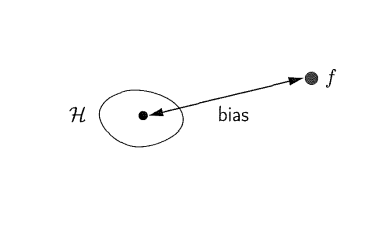
\includegraphics[width=.5\linewidth]{Sesgo-Varianza1}
  \caption{\textbf{Modelo demasiado pequeño}. Como solo hay una hipótesis, $\bar{g}$ y la hipótesis final $g$ son las mismas y por tanto, la varianza 0. El sesgo dependerá de la suerte que hayamos tenido aproximando la función objetivo $f$. \cite{abu2012learning}}
  \label{fig:s-v1}
\end{minipage}%
\hfill
\begin{minipage}{.4\textwidth}
  \centering
  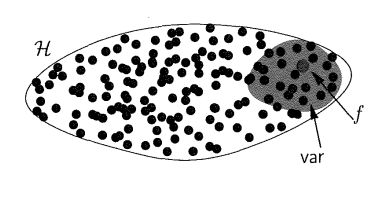
\includegraphics[width=.5\linewidth]{Sesgo-varianza2}
  \caption{\textbf{Modelo demasiado grande}. La función objetivo está en $H$ y muchos conjunto de datos llevarán a la hipótesis $f$ consiguiendo sesgo=0. Sin embargo, la varianza será grande (región gris representada en la figura). \cite{abu2012learning}}
  \label{fig:s-v2}
\end{minipage}
\end{figure}
\subsection{Sobreajuste y regularización}
El \textbf{sobreajuste} (\textit{overfitting} en inglés) ocurre cuando el modelo se ajusta muy bien a los datos de entrenamiento pero no a los de fuera de este conjunto.\\
El sobreajuste puede ocurrir incluso cuando el conjunto de hipótesis contiene sólo funciones que son \textit{mucho más simples} que la función objetivo. \cite{abu2012learning}\\
Para ilustrarlo, tomemos un problema sencillo de regresión unidimensional con cinco puntos en el conjunto de datos. No sabemos la función objetivo así que, como 5 puntos pueden ajustarse por un polinomio de cuarto grado, seleccionamos los polinomios de cuarto grado como el conjunto de hipótesis. La función objetivo es un polinomio de segundo orden con ruido añadido en los puntos de los datos como muestra la siguiente figura:
\begin{figure}[H]
  \centering
  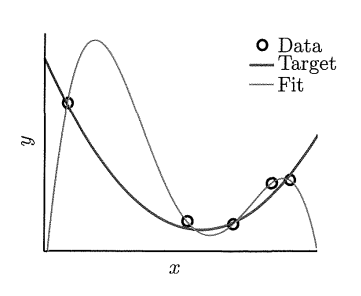
\includegraphics[width=0.4\textwidth]{overfit}
  \caption{Ejemplo de \textit{overfitting}. \cite{abu2012learning}}
  \label{fig:overfit}
\end{figure}
\begin{center}
\end{center}
La linea más clara representa nuestro polinomio de cuarto grado y la oscura, el posinomio de segundo orden objetivo. Con este ajuste, hemos conseguido un error dentro de la muestra nulo pero un gran error fuera de la muestra aproximando la función objetivo.\\\\
La \textbf{regularización} (en inglés \textit{regularization}) es una herramienta para combatir el sobreajuste. Limita el algoritmo de aprendizaje para mejorar el error fuera de la muestra.\\
El algoritmo de regularización utilizado en este trabajo es el conocido como \textit{Lasso} (de sus siglas en inglés \textit{Least Absolute Shrinkage and Selection Operator}) que controla los coeficientes y los limita haciendo que algunos puedan ir incluso a cero lo que da lugar a un procedimiento de estimación y selección de variables simultáneo. Es una forma de mínimos cuadrados penalizada que minimiza la suma de residuos mientras controla la norma $L_{1}$ del vector de coeficientes $\beta$:
\[ argmin_{\beta}(y-X\beta)^{T}(y-X\beta) + \lambda \parallel \beta \parallel_{1} \]
donde $\lambda \geq 0$ indica el grado de limitación que tendrán los coeficientes, que estableciéndolo a 0 se consiguen los mínimos cuadrados ordinarios.
\cite{hans2009bayesian}
\section{Descripción de los modelos utilizados}\label{st:modelos-utilizados}
El problema que se pretende resolver en este trabajo consiste en una predicción de etiquetas, es decir, al uso del aprendizaje supervisado para resolverlo. Dentro del aprendizaje supervisado encontramos varios modelos de gran potencia predictiva como los que describiremos en esta sección.
\subsection{k-Nearest Neighbors}\label{sst:k-nn}
El modelo k-Nearest Neighbours (k-NN) es uno de los modelos más intuitivos y transparentes y se aleja un poco de la idea de aproximar una función ideal para tomar la decisión de clasificación. La idea básica se muestra en la \autoref{fig:k-nn-example}. Se clasificará el vecino desconocido con la clase de los vecinos más cercanos a él, y si hay de varios tipos como en la figura, se puede resolver por simple mayoría o por votación ponderada por distancia, que veremos más adelante. Así que en k-NN se pueden diferenciar dos etapas: primero determinar los vecinos más cercanos y segundo, determinar la clase usando esos vecinos. \cite{padraiddelany2007k}

\begin{figure}[H]
  \centering
  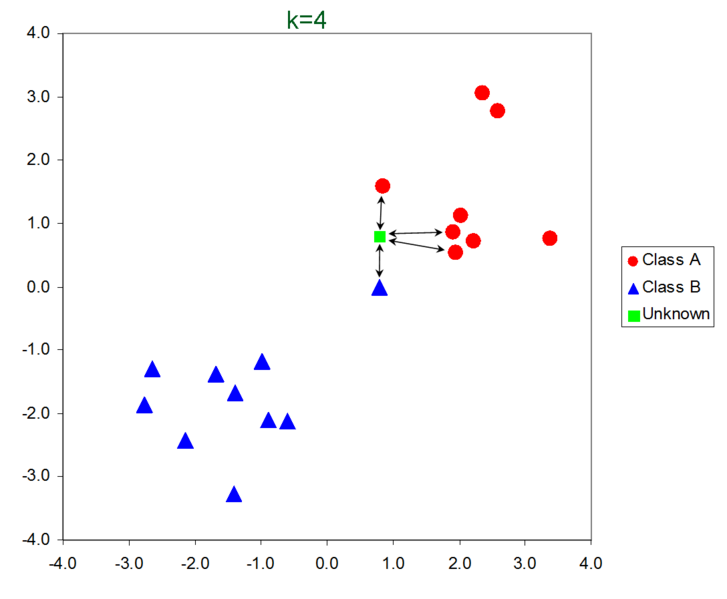
\includegraphics[width=0.4\textwidth]{k-nn-example}
  \caption{Ejemplo de 4-NN.}
  \label{fig:k-nn-example}
\end{figure}
\begin{center}
\cite{peterson2009k}
\end{center}

\subsubsection{Métrica}
Sea $X$=$\lbrace x_{1},...,x_{n} \rbrace$ donde $n=\mid X \mid$ un conjunto de entrenamiento, con x representando las instancias. Las instancias están descritas por un conjunto de variables $F$. Cada instancia de entrenamiento está etiquetada con una etiqueta de clase $y_{i} \in Y$, es decir, la función de etiquetado establece una aplicación biyectiva entre $X$ e $Y$. El objetivo es clasificar un ejemplo desconocido \textbf{$q$}.\cite{padraiddelany2007k}\\
Para cada $x_{i} \in X$ calculamos la distancia como la distancia de :
\[ MD_{p}(\textbf{q},x_{i})= (\sum_{f \in F}  \vert q_{f} - x_{if} \vert ^{p})^{1/p} \quad \cite{inproceedings} \] 
Para p=1 la distancia de Minkowski es la llamada distancia Manhattan, para p=2, la Euclídea y para p=$\infty$ la de Chebyshev. Sus expresiones son las que siguen \cite{inproceedings}:
\[ d^{2}(q,x_{i})= (q-x_{i})(q-x_{i})' \quad Euclídea \]
\[ d(q,x_{i})=\sum_{f \in F}  \vert q_{f} - x_{if} \vert \quad  Manhattan \]
\[ d(q,x_{i})=max_{f \in F} \lbrace \vert q_{f} - x_{if} \vert \rbrace \quad Chebyshev \]

\subsubsection{Votación}
La votación consiste en establecer un criterio para asignar a $q$ una de las etiquetas de $Y$. Esto puede hacerse asignando la etiqueta que tengan la mayoría de vecinos más cercanos a $q$ o también puede establecerse una función de votación. La más usual es establecer la votación en función de la inversa de la distancia entre $q$ y sus vecinos. 
\[ Vote(y_{i}) = \sum^{k}_{c=1} \frac{1}{(d(q,x_{c})^{p}} 1(y_{j},y_{c}) \]
Donde $1(y_{j},y_{c})$ devuelve 1 si las etiquetas son iguales y 0 en caso contrario. En la función, $p$ se suele establecer a 1 pero se puede aumentar o disminuir para cambiar la influencia que tiene la distancia en el voto. \cite{padraiddelany2007k}

\subsection{Regresión Logística}\label{st:reglog}
Para la regresión logística sí que se busca aproximar esa función que se hablaba al principio del capítulo. Para ello, se especifica el conjunto de hipótesis $H$ mediante una forma funcional que todas las hipótesis $h \in H$  comparten. Esta fórmula funcional $h(x)$ se elige dando diferentes \textit{pesos} a cada coordenada de x que reflejan la importancia que esa coordenada tiene en la decisión tomada. Este primer modelo de $H$ se da en el \textit{perceptron}, si llamamos $w$ a los pesos, se diría que el individuo es afectado si \[ \sum_{i=1}^{d}w_{i}x_{i} > umbral \]
\[ \textnormal{y no afectado si } \sum_{i=1}^{d}w_{i}x_{i} < umbral \]
Pudiendo escribir la fórmula más compacta como:
\[ h(x)=sign((\sum_{i=1}^{d}w_{i}x_{i})+b) \]
donde $x_{1},...,x_{d}$ son los componentes del vector x. Si da 1 el individuo es afectado y si da -1 es sano. En el primer caso se le asigna la etiqueta 2 y en el segundo caso la 0, entrando así en el recorrido de nuestro problema. Los pesos y el umbral están determinados por el sesgo $b$ de forma que el individuo está afectado si $\sum_{i=1}^{d} w_{i}x_{i} > -b$. Para simplificar la notación se va a escribir $b$ como el peso $w_{0}=b$ y juntarlo con los demás pesos en un solo vector columna \textbf{w}$=[w_{0},w_{1},...,w_{d}]^{T}$ y también modificamos el vector x como x=[$x_{0},x_{1},...,x_{n}$], donde se le añade la coordenada $x_{0}$ establecida a 1. El espacio de entrada, el dominio, será así
\[ X = \lbrace 1 \rbrace \times \mathbb{R} = \lbrace [x_{0},...,x_{d}]^{T} \vert x_{0}=1, x_{i} \in \mathbb{R} \textnormal{ } \forall i \in \lbrace 1,...,d \rbrace \rbrace\]
y se puede escribir \textbf{$w^{T}x$}=$\sum_{i=1}^{d} w_{i}x_{i}$ y la ecuación de la hipótesis $h(x)$ quedaría:
\[ h(x) = sign(w^{T}x) \]
\cite{abu2012learning}\\
La regresión logística se separa de la clasificación lineal en que la decisión que toma no es binaria sino que tiene como salida una \textbf{probabilidad}, un valor entre 0 y 1. La clasificación lineal usa un umbral basado en $w^{T}x$, $h(x) = sign(w^{T}x)$ mientras que la regresión lineal no usa ningún umbral $h(x) =w^{T}x$. En la regresión logística se busca algo intermedio que se consigue con la función \textit{logística} $\theta(s)=\frac{e^{s}}{1+e^{s}}$ cuyo valor está entre 0 y 1, quedando \[ h(x)=\theta(w^{T}x) \] cuyo valor se interpreta como la probabilidad de que ocurra un suceso binario. Se está tratando de aprender la probabilidad de que el individuo esté afectado por el trastorno y eso depende de la entrada x. La función objetivo es por tanto $f(x)= \mathbb{P} [y=1 \vert x]$ pero los datos no dan el valor de $f$ de forma explícita sino observaciones de ésta (individuos que ya se sabe que están afectados). Por tanto, los datos están generados por una distribución objetivo $P(y \vert x)$,
\[P(y \vert x)=\spalignsys{
f(x) \textnormal{      para }  y=1;
1-f(x) \textnormal{   para }  y=-1}\]
así que para aprenderlo se necesita una medida de \textbf{error} que indique cómo de parecida es la $h$ a la función objetivo $f$ en términos de las etiquetas de las observaciones.\cite{abu2012learning}\\
Por tanto se tiene que el conjunto de muestras $X=\lbrace x_{1},...,x_{N} \rbrace$ es una muestra aleatoria simple pues los individuos son tomados de forma independiente y están idénticamente distribuidos.\\
El error en este modelo se basa en la idea de cómo es de "probable" que se consiga la salida $y$ de la entrada $x$ si la distribución objetivo $P(y \vert x)$ estuviera definida por nuestra hipótesis $h(x)$. Esto sería:
\[P(y \vert x)=\spalignsys{
h(x) \textnormal{      para }  y=1;
1-h(x) \textnormal{   para }  y=-1}\]
Sustituyendo $h(x)$ por su valor $\theta(yw^{T}x)$ y usando que $1-\theta(s)=\theta(-s)$, probado a continuación, queda \[ P(y \vert x)=\theta(yw^{T}x) \]
\begin{proposicion}La función logística $\theta: \mathbb{R} \rightarrow [0,1] \textnormal{, } \theta(s)=\frac{e^{s}}{1+e^{s}}$ tiene la propiedad simétrica: \[1-\theta(s)=\theta(-s) \textnormal{ } \forall s \in \mathbb{R} \]
\end{proposicion}
\begin{proof}
Se toma $s \in \mathbb{R}$ y se tiene que $1-\theta(s)=1-\frac{e^{s}}{1+e^{s}}$, multiplicando numerador y denominador por $e^{-s}$ en la fracción queda $1-\frac{1}{1+e^{-s}}$, realizando la resta se tiene $\frac{1+e^{-s}-1}{1+e^{-s}}$ y simplificando queda $\frac{e^{-s}}{1+e^{-s}}=\theta(-s)$, como se quería demostrar.
\end{proof}
Las observaciones $(x_{1},y_{1}),...,(x_{N},y_{N})$ son tomadas independientemente así que la probabilidad de obtener todas las salidas $y_{n}$ en los datos desde la correspondiente muestra $x_{n}$ sería el producto \[ \prod_{n=1}^{N}P(y_{n} \vert x_{n}) \]
El método de la máxima verosimilitud (\autoref{st:emv}) selecciona la hipótesis $h$ que maximiza esta probabilidad. Equivalentemente, se puede minimizar la siguiente expresión más conveniente para la medida del error:
\[ \frac{-1}{N}ln \left(\prod_{n=1}^{N}P(y_{n} \vert x_{n})\right) = \frac{1}{N}\sum_{n=1}^{N}ln \left(\frac{1}{P(y_{n} \vert x_{n})} \right) \]
dado que la expresión '$\frac{-1}{N}ln(\cdot)$' es una función monótona decreciente y sustituyendo el valor de la probabilidad, estaríamos minimizando
\[ \frac{1}{N}\sum_{n=1}^{N}ln \left(\frac{1}{\theta(y_{n}w^{T}x_{n})} \right) \]
con respecto al vector de pesos $w$. Y como estamos minimizando, nos lleva al concepto de error. Sustituyendo la forma funcional de $\theta(y_{n}w^{T}x_{n})$ produce el error dentro de la muestra para la regresión logística,
\[ E_{in}(w) = \frac{1}{N}\sum_{n=1}^{N}ln \left(1 + e^{-y_{n}w^{T}x_{n}} \right) \textnormal{.}\]
Para minimizarlo, usamos el \textbf{gradiente descendente} en su versión \textbf{estocástica}. Repasaremos antes la versión no estocástica.\\
El gradiente descendiente es una técnica para minimizar funciones de clase  $C^{2}$ como $E_{in}(w)$ en regresión logística. Como $E_{in}$ es una función convexa, esta técnica siempre alcanzará el mínimo absoluto empiece donde empiece. Supongamos que empezamos en $w(0)$ y tomamos un paso hacia 'abajo' de tamaño $\eta$ con la dirección de un vector $\hat{v}$. Como $\eta$ es pequeña, usamos la serie de Taylor de primer orden, quedando el diferencial de $E_{in}$ como
\[ \Delta E_{in} = E_{in}(w(0)+ \eta \hat{v}) -E_{in}(w(0)) = \eta \nabla E_{in} (w(0))^{T} \hat{v} + O(n^{2}) \geq -\eta \parallel \nabla E_{in}(w(0)) \parallel \]
donde hemos ignorado un pequeño término $O(\eta^{2})$. La igualdad se cumple si, y solo si,
\[ \hat{v}=-\frac{\nabla E_{in}(w(0))}{\parallel \nabla E_{in}(w(0)) \parallel } \textnormal{,} \]
que indica la dirección al mayor decrecimiento de $E_{in}$ para un tamaño $\nabla$ dado. \cite{abu2012learning}
\begin{figure}[H]
  \centering
  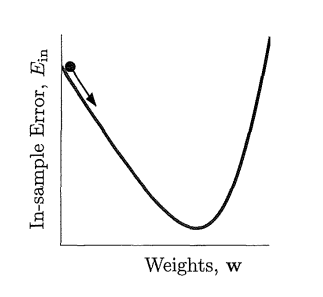
\includegraphics[width=0.4\textwidth]{GradDesc1}
  \caption{Un paso hacia abajo de tamaño $\eta$ con dirección $\hat{v}$.}
  \label{fig:GradDesc1}
\end{figure}
\begin{center}
\cite{abu2012learning}
\end{center}

La longitud de ese paso que tomamos es importante en esta técnica pues define el comportamiento que tiene como puede verse en los siguientes ejemplos visuales:
\begin{figure}[H]
\minipage{0.32\textwidth}
  \includegraphics[width=\linewidth]{etapequeño}
  \caption{$\eta$ muy pequeña.} \label{fig:etapequeño}
\endminipage\hfill
\minipage{0.32\textwidth}
  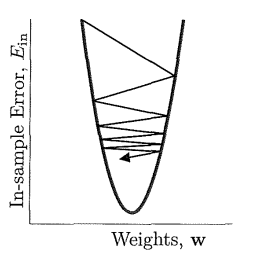
\includegraphics[width=\linewidth]{etagrande}
  \caption{$\eta$ muy grande.} \label{fig:etagrande}
\endminipage\hfill
\minipage{0.32\textwidth}%
  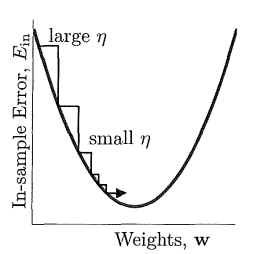
\includegraphics[width=\linewidth]{etabien}
  \caption{$\eta$ correcta.} \label{fig:etabien}
\endminipage
\end{figure}
Cuando $\eta$ es muy pequeño, se hace ineficiente llegar al mínimo local y cuando es grande es posible que incluso aumente $E_{in}$.\\
Con esto, podemos definir el algoritmo de regresión logística usando gradiente descendiente:
\begin{lstlisting}[escapeinside={(*}{*)}]
Inicializar los pesos en el paso t=0 a w(0)
para t=0,1,2... hacer{
	Computar el gradiente
	(* $ g_{t}=-\frac{1}{N}\sum_{n=1}^{N} \frac{y_{n}x_{n}}{1+e^{y_{n}w^{T}(t)x_{n}}} $*)
	Establecer la direccion del movimiento, (* $v_{t}=-g_{t}$ *)
	Actualizar los pesos (* $w(t+1)=w(t)+\eta V_{t}$ *)
	Iterar al siguiente paso hasta alcanzar la parada
}
Devolver los pesos finales w
\end{lstlisting} 
Pasamos ahora sí al \textbf{gradiente descendiente estocástico}.\\
Esta vez, en vez de considerar el gradiente completo en todos los $N$ puntos del conjunto de entrenamiento, consideramos una versión estocástica del gradiente. Primero, tomamos un punto del entrenamiento aleatorio de forma uniforme $(x_{n},y_{n})$ y consideramos solo el error en ese punto, en caso de la regresión logística
\[e_{n}(w)=ln(1+e^{-y_{n}w^{T}x_{n}}) \textnormal{.}\]
Y usamos el gradiente en este error para actualizar los pesos:
\[ \nabla e_{n}(w) = -\frac{y_{n}x_{n}}{1+e^{y_{n}w^{T}x_{n}}} \]
actualizamos con ello los pesos $w \leftarrow w -\eta \nabla e_{n}(w)$. Así, obtenemos que la esperanza del cambio de los pesos, como $n$ la tomamos de forma aleatoria de {$1,...,N$}, es la misma que para el gradiente descendiente:
\[ -\eta \frac{1}{N} \sum_{n=1}^{N} \nabla e_{n}(w) \textnormal{.} \]
La diferencia radica en una componente aleatoria que tiene en cada actualización de pesos, que a la larga se cancela y conseguimos un coste computacional más barato en un factor de $N$. \cite{abu2012learning}\\
\subsection{Árboles de decisión}
Son un modelo de aprendizaje no paramétrico usado para clasificación y regresión (para clasificación en este trabajo). Es un modelo fácil de entender y eficiente (eficiencia logarítmica a la hora de predecir) pero tiende al sobreajuste. \cite{scikit2021dt}\\
Hay numerosos algoritmos para este modelo y el que se usa en la implementación de \textit{scikit-learn} es una versión optimizada del llamado \textbf{CART} (por sus siglas en inglés \textit{Classification and Regression Trees}). Su metodología consiste en tres partes:
\begin{itemize}
 \item 1. Construcción del árbol \textit{máximo}.
 \item 2. Elección del tamaño del árbol. Que se puede hacer con validación cruzada. \cite{timofeev2004classification}
 \item 3. Clasificación de nuevos datos usando el árbol construido.
\end{itemize}
\cite{timofeev2004classification}\\
Construir el árbol máximo es la parte que lleva más tiempo. Sea $t_{p}$ un nodo padre y $t_{l},t_{r}$ sus nodos hijos de la izquierda y la derecha respectivamente. Consideremos la muestra de entrenamieno como una matriz variable $X$ con $M$ números de variables $x_{j}$ y $N$ observaciones. Sea el vector de etiquetas $Y$ compuesto de $N$ observaciones con $K$ clases.\\
El árbol de clasificación se construye de acuerdo a la \textit{regla de separación} donde los cada vez los datos se separan en dos partes con la máxima homogeneidad. Si llamamos $x_{j}^{R}$ el mejor valor de separación de la variable $x_{j}$ nos queda como regla de separación:
\begin{figure}[H]
  \centering
  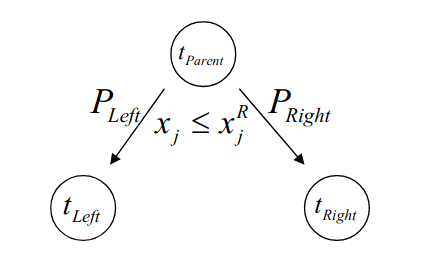
\includegraphics[width=0.4\textwidth]{ReglaSeparacion}
  \caption{Algoritmo de separación de CART. \cite{timofeev2004classification}}
  \label{fig:k-nn-example}
\end{figure}
\begin{center}
\end{center}
La homogeneidad máxima de los nodos hijos se define por la llamada \textit{función de impureza i(t)} que se definirá un poco más adelante. Como la impureza del nodo padre es constante para cada posible separación, la máxima homogeneidad de los hijos izquierdo y derecho será equivalente a la maximización de la diferencia en la función de impureza $\Delta i(t)$:
\[ \Delta i(t) = i(t_{p})-E[i(t_{c})] \]
donde $t_{c}$ indica ambos nodos hijos. Si $P_{l},P_{r}$ son las probabilidades de los nodos izquierdo y derecho, obtenemos:
\[ \Delta i(t)= i(t_{p}) - P_{l} i(t_{l}) - P_{r} i(t_{r}) \]
Por tanto, en cada nodo CART soluciona el siguiente problema de optimización:
\[ \argmax_{x_{j} \leq x_{j}^{R},j=1,...,M}[i(t_{p}) - P_{l} i(t_{l}) - P_{r} i(t_{r})] \]
\cite{timofeev2004classification}\\
Ahora sí, definimos la función de impureza. La regla más usada es la de \textbf{Gini} que usa la siguiente función de impureza:
\[ i(t) = \sum_{k \neq l} p(k \vert t)p(l \vert t) \]
donde $k,l \in {1,...,K}$ son índices de las clases y $p(k \vert t)$ la probabilidad condicional de la clase $k$ condicionada a que estamos en el nodo $t$. Así, la diferencia $\Delta i(t)$ queda:
\[ \Delta i(t) = -\sum_{k=1}^{K} p^{2}(k \vert t_{p}) + P_{l} \sum_{k=1}^{K} p^{2}(k \vert t_{l}) + P_{r} \sum_{k=1}^{K}p^{2}(k \vert t_{r}) \]
Por lo tano, Gini soluciona el siguiente problema de optimización:
\[ \argmax_{x_{j} \leq x_{j}^{R},j=1,...,M} \left[ -\sum_{k=1}^{K} p^{2}(k \vert t_{p}) + P_{l} \sum_{k=1}^{K} p^{2}(k \vert t_{l}) + P_{r} \sum_{k=1}^{K}p^{2}(k \vert t_{r}) \right] \]
buscará en la muestra de entrenamiento la mayor clase y la aislará del resto. Funciona bien para datos con ruido.\\
Para la parte de clasificación de nuevos datos, se usa el árbol ya construido y a un nuevo dato se le asigna la \textit{clase dominante} del nodo terminal (el último nodo del árbol donde queda el nuevo dato) que es la clase con el mayor número de observaciones.\cite{timofeev2004classification}\\
\subsection{Máquinas de soporte vectorial}
Las máquinas de soporte vectorial (\textbf{SVM} por sus siglas en inglés) son un algoritmo de aprendizaje automático supervisado que es efectivo para conjuntos de datos de alta dimensionalidad y suele ser usado por ello para problemas de clasificación biológica \cite{10.1093/bioinformatics/btw498} \cite{cortes1995support}.\\















\endinput











